\section{Vampirism and Vampires}

\begin{quotex}
This essay by \textbf{Julius Evola} was originally published in the journal ``Roma" on 6 September 1973 under the title ``Il vampirismo ed i vampiri".

This topic is certainly even more relevant today that it was 40 years ago. Although we don't agree this is the last word that can be said on the topic of vampirism, we will allow Evola to speak for himself and bring in other issues either in the comments or in another post. This perhaps explains the expression \emph{ride the tiger}. 
\end{quotex}

Recently the ``vampire" theme has acquired some popularity through various publications, beginning with Bram Stoker's famous novel \emph{Dracula}. Some have given that interest a psychological and psychoanalytical interpretation. The idea of the vampire in itself, however, cannot entirely be reduced to superstition and extravagant fantasy. To be put aside, however, is vampirism as grossly physical, with blood taken from the victim by the vampire, sometimes with the goal of prolonging his own life.

Instead, vampirism could be considered in its psychic character and we could bring attention to the phenomena which often is the issue both in popular belief, and in ethnology. We cannot overlook even whatever there is in the childish fables as the type of the ``werewolf" and which in ethnology is designated as lycanthropy.

It is about the idea that a human being can in a certain way split in two and that his double can assume an animal appearance and manifest corresponding behaviors. What can there be in that which is real?

In terms of principle, we can respond affirmatively, referring to the following framework. True human evolution must be conceived as the self-differentiation of the human type by means of the exclusion, in the course of the history of the species, of animal possibilities that he included in himself, that he left outside of himself like the wake of a boat, and that already had been realized and established in given animal species. Now, we can conceive a human type in which this differentiation was not sufficiently determined. That occurs especially among primitive and savage populations which are at the stage of so-called totemism, the totem being both the progenitor of a given tribe, as well as the god or demon of an animal species, through which the members of that tribe consider themselves, e.g., as leopard-men, wolf-men, bear-men, and so on.

Now, theoretically, one cannot exclude that in a being, whose personality is not stable enough, this animal potentiality creates, even today, an irruption and is manifested in a corresponding way. It is not the case that the being is then transformed materially or physically into an animal, as in the fantastic case of Dr. Jekyll. One should think instead of a scission of the personality (phenomena, certainly verified by psychology, as in ``multiple personalities") which is developed in analogous terms to phenomena, also verified positively, as in ``ectoplasm": they are the formations that, in extrasensory seances, drew their origin from the psychic-physical substance of the medium.

An ectoplasm that assumes the transitory form of an animal nature through the regressive irruption of a force of animality: this would therefore be the possible explanation of phenomena like the werewolf and similar forms, possibly including vampiric forms if the animal manifestation includes such behavior. Therefore, it is not a question of a dead person becoming a vampire nor of a person who transform himself into an imaginary animal. From the material gathered by ethnology, there seem to be actual cases of certain persons who are found in a state of deep sleep or catalepsy, while one of their doubles moves about and is seen by others.

The double, as the ectoplasm of the medium, maintains a certain mysterious connection with the subject, because it means that a wound produced in that image would be reproduced in the dormant or cataleptic body.

Finally, we could mention the phenomena of bilocation, and depending on whether one is disposed to admit it on a higher plane (bilocation of certain Christian saints, Islamic sheiks, Hindu yogis, etc.), they could also come into question as explicative elements for this rather sinister field.

Naturally, in werewolves and similar creatures, the possible manifestations do not have the erotic setting that certain ``dark" literature often likes to attribute to the vampire. Through this setting, we have to move into a rather different domain, that of an essentially psychic vampirism that can be real that is confirmed in more than a few traditions, which sometimes even indicate the technique to actualize it.

Moreover, ethnology has recorded the belief that certain shamans have the power to vampirize living beings to the point of reducing them to a type of bare nothings\footnote{I presume ``zombies".}: they seem to have been left traces of that in the black practices of the Voodoo of Haiti. Regarding properly erotic vampirism it is instead the case when the subtle vital force of a woman is fed with the goal of strengthening one's own vitality. That seemed to be the case in the Old Testament, with King Solomon\footnote{I think he means King David.} who lay down with naked young girls, ``without knowing them": all the more that an analogous procedure is likewise attested to both in central Asia and ancient China.

\begin{wrapfigure}{rt}{.3\textwidth}
 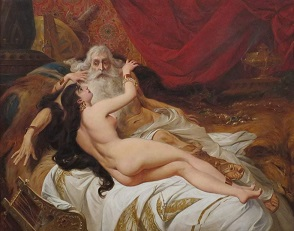
\includegraphics[scale=.5]{a20130106VampirismandVampires-img001.jpg} 
\end{wrapfigure}

Regarding the former, Alexandra David-Neel who stayed there for quite a while, recounts that one of the methods ``to increase one's own life" and maintain one's own youth would consist in using young women to come to orgasm without however participating in the pleasure. More or less the same procedure is again found in ancient operative Chinese Taoism, in the play of the Dragon with the Tiger (the Dragon representing man, the Tiger the young woman), meant to guarantee ``eternal life" to the one ``who has knowledge". Here, sometimes, it would seem to be about a pure masculine vampirism (having as its object not blood but a vital subtle substance) not only because, rather unfairly, the young women should be kept in the dark about the hidden goal of the union for fear that, by knowing it, they could take the lead, inverting the roles and exploiting the man who would like to vampirize them, but also because it is recommended to use different ones sequentially, one text saying that the best result is obtained when one is matched with as many as ten girls in one night.

That, however, does not represent a barely credible masculine \emph{tour de force} (especially if the designation of the woman as ``tiger" was not just a manner of speaking), because, at the same time, it is prescribed not to ejaculate (``rigid organ without ejaculation"), which relates to what the method required to strengthen his own life, again evidently requiring the renunciation, on the man's part, of the pleasure that man experiences when he pours himself without reservation into the woman's flesh.

This is, more or less, all that can be said about vampirism, while also bringing back ideas from a rather distant domain of ordinary existence, but not for that reason, by way of principle, deprived of every reality.



\flrightit{Posted on 2013-01-06 by Cologero }

\begin{center}* * *\end{center}

\begin{footnotesize}\begin{sffamily}



\texttt{Janus on 2013-01-06 at 18:37 said: }

Is the sexual practice of increasing vitality here distinguished from the practices used in Tantra, where the practice of the man either withholding climax or experiencing orgasm without ejaculation is also used, or are they the same thing? It seems as though the mere concept of increasing ones ``life" or ``vitality" would constitute a misunderstanding or degeneration of Traditional practices, which focus on rising to a new form of life and existence. 

Gandhi also lay with young women in this way, yet I find it hard to believe that he or Evola are urging us to become ``vampires" (even in this proper sense of the word). The link between totemism and the shamanic animal cult or animal-man certainly seems in line with what we know today about tribal practices.


\hfill

\texttt{Cologero on 2013-01-06 at 20:48 said: }

Guenon seems to take your point of view, Janus. What Evola calls ``operative" Taoism would be dismissed as merely ``magic" by Guenon. ``Laying with young women" should be understand in the alchemical sense, and those who need to do it corporeally are on the same level as the ``puffers" (i.e., those who confuse alchemy with chemical experiments). In ``Man and his becoming", Guenon specifically addresses the meaning of ``longevity" in Taoism, which is the prolongation of human individuality, not necessarily as bodily existence.


\hfill

\texttt{Jason-Adam on 2013-01-06 at 21:08 said: }

As someone who was raised with beliefs of pre-revolutionary Europe – I am find this article hard to even read, what separates this from porn ? Sex magic is Satanic as far as I'm concerned…..


\hfill

\texttt{Logres on 2013-01-06 at 22:56 said: }

Jason, I share your upbringing and general outlook. Yet many of the celibates had a sort of higher spiritual dynamic that was obviously far removed from the pornographic:

St. Cyprian and Juliana – http://en.wikipedia.org/wiki/Cyprian\_and\_Justina

Or Heloise, and Abelard.

Also, Weor writes on Perfect marriage: http://www.anael.org/descargas/books/matrimony.pdf (which I have yet to read entirely).

At it's best, even the rite of Christian marriage is an exoteric outworking of certain basic spiritual truths, one of which is that man and woman practice giving of themselves, faithfully, to only one other person, over a lifetime. They are essentially practicing the recognition of their polar being. According to Bo-Yin-Ra, this practice (even if someone not your polar being – which are the human odds anyway) will bear fruit towards recognizing your true other self.


\hfill

\texttt{Janus on 2013-01-06 at 23:20 said: }

That makes sense. To my knowledge neither Rome nor Christendom used the literal sexual practices described, and in Christendom at least sex seems to fall into the realm of the man and wife ``becoming one flesh" (or exemplifying both masculine and feminine in their entirety and ultimate union). Thank you for the clarification.


\hfill

\texttt{Cologero on 2013-01-07 at 07:28 said: }

Interesting point, Jason-Adam, given that Evola himself claims to hold the values of pre-revolutionary Europe. As a thought experiment, let's look at understanding the phenomena that Evola mentions from a different point of view.

The feminine represents the soul, whose symbol is the tiger. As we are, our souls are unruly, unpredictable, and even dangerous to our eternal life (i.e., ``longevity"). We can try to ride the tiger just to retain balance and sanity. Ideally, however, the soul is virginal. That means it is passive and receptive to the Spirit (Intellect and Will), thus directed by it. As virginal, it is not full of ``wandering influences", or random thoughts absorbed unconsciously or uncritically from other men.

The number 10, the sum of 1 through 4, represents a complete cycle, so the 10 virgins (haven't we heard that somewhere else in another context?) represent a complete cycle in the mind. The microcosm is the macrocosm, and this is seldom remembered in talks about the cosmic cycle. So, in consciousness, we also have to traverse the entire cycle, from the primordial state, through the fall of the Kali Yuga, a re-awakening, and the deliverance. Notice how this follows the trajectory of the Divine Comedy, another work explicitly motivated by the ideal of the feminine without ``carnal knowledge", whereby a man has to attain self-knowledge of the faults in his soul, purge them, and attain Heaven.

The animal totems are also interesting. The West has always taught that we have an ``animal" soul, although this doctrine is poorly understood and developed. Assuming that sorcerers can create the illusion of a animal form through ``ectoplasm", just as in a seance there is the illusion of communication with the dead, it is not normally something anyone is too concerned about. The real problem is that animal natures can manifest in actual men; this is too obvious to expand on at this point as I am sure many examples can be provided.

As for the vampire. The real issue is not their existence, but rather why, starting post-revolution and reaching a fever pitch in our day, is there this fascination with the vampire. Obviously, it is the irruption into the common soul life in the West of some deep disturbance; this explains the eroticism.

It would seem, then, that there are now appearing human beings in a state of devolution and the vampire represents the totem. Rather than animals, which are really morally neutral, this new totem is something far more sinister. As E Michael Jones points out, the vampire attains eternal life by drinking the blood of his followers. The contrast is too obvious to state.


\hfill

\texttt{Mihai on 2013-01-07 at 09:30 said: }

The entire western world seems to be completely immersed in an entertainment based around a degenerate and completely out of control sexuality driven beyond the point of obsession, on the one hand, and an equally disturbing obsession with extreme violence, horror literature and movies, sinister images, gore, destruction etc., on the other hand.

It is not hard to intuit the causes. At this point of the Kali Yuga, what Guenon called ``fissures in the Great Wall" have developed into entire gaps, where demonic influences from the lower psychic regions have launched a general assault and invaded a large part of the consciousness of the (post)modern individual- left completely unguarded thanks to evolutionism and relativism. 

After all, why question the value of your thoughts and impulses is value is something relative ? Plus, if we are all automatically ``evolving", then there is no reason to worry, is it ?

Perhaps my past articles on postmodernism deserve an additional part along the lines above.


\hfill

\texttt{Logres on 2013-01-07 at 10:24 said: }

Mihai, I'm glad you've used Upton as a resource : a couple of years ago, I became fascinated with UFOs, as I was convinced both from personal experience (I have seen something preternatural a long time ago) and talking to others (otherwise respectable people) that the phenomenon was not capable of being dismissed. I read about medieval accounts, as well, and what struck me was the difference (modern accounts being highly ``technological"). It occured to me demons might manifest in the form considered most useful for fear and false worship – what else do we worship today, but technology (at least at a common level)? Upton confirmed all that when I stumbled over him, and it was good to see you put these things in context, to which Cologero's account here also adds a great deal.


\hfill

\texttt{Mihai on 2013-01-08 at 04:47 said: }

Fr. Seraphim Rose is also a good resource concerning these phenomena- Upton elaborated very much on Rose's ideas. 

What you wrote is true and there is on more thing to take into account: that is science-fiction literature- not only the cheap one, but also the more elaborate writing, such as those of Asimov or Herbert. The world they portray there has many things in common with many new-age theories. 

For example, in Dune, we have a futuristic humanity which has ``evolved" to the point of colonizing the Universe, ruled by a sort of an agnostic elite that resembles the medieval order, minus the spiritual. In fact, humanity has adopted a sort of syncretistic religion built up of bits and pieces from all world religions and where high technology is combined with ``orders" who specialize in manipulating psychic powers and manipulate events through these powers as well as genetic engineering. 

Also, even if I've never read a single book by Asimov, I know as a fact that, even though he was a stark and militant (materialist) atheist, his books are full of reference to psychic powers and sorcery.

We have here all the ingredients of the type of society that post-modern theorists dream of.

It is really hard to ignore the possibility that this kind of authors can easily be unconscious agents for spreading a certain kind of worldview, especially considering the fact that, in popular opinion, what is today sci-fi, may become tomorrow reality.


\hfill

\texttt{Saladin on 2013-01-08 at 20:34 said: }

As an Oriental, it is interesting to see, just based on the number of comments here, how phenomena (weird or otherwise) fascinates my Occidental brethren! UFOs, Werewolves, Vampires, … truly make this colorful world of ours more colorful. But alas, they remain phenomena!

This fits well with what Janus said below: ``It seems as though the mere concept of increasing ones ``life" or ``vitality" would constitute a misunderstanding or degeneration of Traditional practices." Indeed my brothers, it's not the number of years of the human life that counts … ``Der Mensch ist etwas, das überwunden werden soll"

\texttt{Cologero said: " As E Michael Jones points out, the vampire attains eternal life by drinking the blood of his followers. The contrast is too obvious to state."}

WoW! That had not occurred to me before! Clear example of ``inversion" by Counter-Initiation!


\hfill

\texttt{Senko on 2013-01-08 at 23:52 said: }

Mihai and Logres, both my father and I have seen UFO's and we both can attest that the vision was accompanied by a sense of fear and of a dark presence. In my case, when I saw it, the only sci-fi material I had been exposed too was Star Wars, coincidentialy the UFO looked like a Star Destroyer.

Upton work is fantastic, also Frater Rose. I have found Orthodox text in general, but Rose and Olivier Clement in general to provide not only a good many themes for contemplation but a lot of practical/ operative insights.


\hfill

\texttt{Logres on 2013-01-09 at 10:11 said: }

Senko, immediately prior to my experience, I had an impending sense of doom/dread which was so overwhelming it actually polarized me towards God (what else to do?) : several seconds later, I saw what I saw.


\hfill

\texttt{Jason-Adam on 2013-01-10 at 09:29 said: }

It seems to me though that whereas writers such as Dante used the language of romance as spiritual allegory, or arcana to use a better word perhaps, Evola seems to actually mean sex as a literal act. If I understand him correctly he would have had no problems having a one night stand with Beatrice thus rending null the whole notion of love from afar that made the Middle Ages so beautiful and inspiring…..though then again it can be argued Evola might have been trying to shock people ? His discussion of the degeneracy of modern marriage in Ride the Tiger was spot on and a Catholic priest couldn't have said it any better how little people think of the sacrament these days…..


\hfill

\texttt{Cologero on 2013-01-10 at 23:37 said: }

The odds of finding your polar being? They may be pretty good. The odds of recognizing her as such? Should be the same, but probably is not.


\hfill

\texttt{Aleksandar Gueric on 2016-01-14 at 07:25 said: }

Apparently, Baron did practiced some form of erotic vampirism on young women of Rome in his later years, according to one eyewitness, but who knows. I take those gossips with the grain of salt. In any case, this literal sexual practice is just one smaller aspect of "ride the tiger" concept


\hfill

\texttt{Sparrow on 2016-09-01 at 03:38 said: }

The vampire, or werewolf, always symbolized to me someone who has rejected the nous and wholly embraced what Schopenhauer termed the ``will to live." there are plenty of people like that in the modern world, but they are generally content to live more like sheep, contenting themselves with grazing, while the ``wolf-man" and vampire were more active and possessed some modicum of will (no matter how crude or animalistic) with which to pursue eternal life, which they identified with telluric and not solar life.


\end{sffamily}\end{footnotesize}
